\documentclass[11pt]{article}
\usepackage{amssymb}
\usepackage{amsmath}
\usepackage{fullpage}
\usepackage{enumerate}
\renewcommand{\theenumi}{\roman{enumi}}
\usepackage{color}
\definecolor{Purple}{rgb}{.9,0,.9}
\newcommand{\solution}[1]{\textcolor{Purple}{\\Solution: #1}}  %Solution
\newcommand{\C}[1]{\ensuremath{\mathord{\rm #1}}}
\newcommand{\pair}[1]{\ensuremath{\mathopen{\langle}#1\mathclose{\rangle}}}
\newcommand{\lng}[1]{\ensuremath{\mathopen{|}#1\mathclose{|}}}
\newcommand{\card}[1]{\ensuremath{\mathopen{|\!|}#1\mathclose{|\!|}}}
\newcommand{\manyone}{\ensuremath{\leq_m^p}}
\newcommand{\pmli}{\ensuremath{\leq_{m,\mathord{\rm li}}^p}}
\newcommand{\ponem}{\ensuremath{\mathrel{\leq_m^{p/1}}}}
\newcommand{\ponett}{\ensuremath{\mathrel{\leq_{1-\mathord{\rm tt}}^{p/1}}}}
\newcommand{\ptt}{\ensuremath{\mathrel{\leq_{\mathord{\rm tt}}^p}}}
\newcommand{\pktt}{\ensuremath{\mathrel{\leq_{k-\mathord{\rm tt}}^p}}}
\newcommand{\pttk}[1]{\ensuremath{\mathrel}{\leq_{#1-\mathord{\rm
        tt}}^p}}
\newcommand{\pmhat}{\ensuremath{\mathrel{\leq_{\hat{m}}^p}}}
\newcommand{\pmhatli}{\ensuremath{\mathrel{\leq_{\hat{m}\mathord{\rm
          ,l.i.}}^p}}}
\newcommand{\pmhathonest}{\ensuremath{\mathrel{\leq_{\hat{m},\mathord{\rm honest}}^p}}}
\newcommand{\PNP}{\C{P}^{\C{NP}}}
\newcommand{\pT}{\ensuremath{\mathrel{\leq_T^p}}}
\newenvironment{proof}{\vspace*{1em}\noindent{\bf Proof.}}{\hfill$\Box$}
\newtheorem{theorem}{Theorem}
\newtheorem{lemma}[theorem]{Lemma}
\newtheorem{corollary}[theorem]{Corollary}
\usepackage{graphicx}
\graphicspath{ {./} }
%\setlength{\parindent}{0cm}
\title{Identifying Pathway Modules from High Throughput Genetic Interaction Data using Simulated Annealing}
\author{Jeremy Colebrook-Soucie, Quinn Collins}


\newtheorem{definition}[theorem]{Definition}


% NOTE! Affiliations placed here should be for the institution where the
%       BULK of the research was done. If the author has gone to a new
%       institution, before publication, the (above) affiliation should NOT be changed.
%       The authors 'current' address may be given in the "Author's addresses:" block (below).
%       So for example, Mr. Fogarty, the bulk of the research was done at UIUC, and he is
%       currently affiliated with NASA.

\begin{document}

\maketitle

% Head 1

% \section{Abstract}


\section{Introduction}

\par In this paper, we explore simulated annealing as an alternative method for detecting patterns from high throughput genetic interaction data. This work has been done as an extension of the genecentric package and the LocalCut method defined in Leiserson \textit{et al} (Leiserson 2011). We also touch upon subsequent verification techniques.

\par High throughput genetic interaction data can be represented as a weighted, undirected graph, in which each vertex is a gene and each edge is how positive or negative the genetic interaction between the two genes is. Thus, we can identify genes that belong in the same pathway because the genes are likely to have positive genetic interactions with one another. We can also identify genes that belong in a related pathway, because the genes in one pathway will have many negative genetic interactions with another related pathway.  

\par We represent related genetic pathways as BPMs (between pathway models), which are each composed of two modules of genes. Each module represents a possible gene pathway, and each BPM represents 2 possible related gene pathways. Thus, we aim to maximize the positive edge weights in each module, and negative edge weights between modules in the same BPM. 

\par We apply simulated annealing to high throughput genetic interaction data to generate possible BPMs. Applying simulated annealing allows us to generate "bad" BPMs early on, that might not have strong positive interactions within each module and strong negative interactions between modules, in order to explore the sample space. As the process continues, we gradually move towards better BPMs until we find a set of BPMs that have weights within and between modules that we consider "good". Thus, simulated annealing allows us to explore a large possible sample space and come up with a probable solution. 

\section{Data}

The data that we examined and performed our analysis on was created by Tufts' Bioinformatics and Computational Biology Research Group. This dataset was based on Collins \textit{et al.}'s genetic interaction map on protein complexes involved in yeast chromosome biology from the Krogan Lab Interactome Database[Collins 2007]. The format of this dataset was consistent with that required by the genecentric package [Leiserson 2011, Gallant 2013]. 
\section{Methods}
\subsection{Simulated Annealing}
\par Simulated annealing is a hueristic that is used for solving optimization problems with a very large sample space. Its function is analogous to the physical process of annealing, where a metal is heated and then slowly cooled in order to remove imperfections. When the metal is hot, the smith can make large changes to it. However, as it cools, only smaller and smaller changes can be made. 

\par Let us define the following terminology. 

\begin{definition}
{\bf Objective Function} The objective function is a function from an element in the sample space to the real numbers. Simulated annealing attempts to minimize this function.
\end{definition}
 
\begin{definition}
{\bf Permutation} how simulated annealing gets from one valid point in the sample space to another. In general, such permutations are simple, random changes in a solution. 
\end{definition}


\begin{definition}
{\bf Temperature}  defines how willing simulated annealing is to accept worse solutions. When temperature is high, simulated annealing has a large probability of accepting a solution that is worse than the previous candidate. However, when the temperature is low, simulated annealing will accept worse solutions with lower and lower probabilties. 
\end{definition}

\par Simulated annealing works by exploring the sample space, with the end goal of minimizing the objective function of the final solution. It begins with a very high temperature, which exponentially decays over a fixed number of total iterations. At every iteration, it generates a new solution based on the previous solution. It then  evaluates this new solution and then decides whether or not to accept it based on how it compares to the previous solution and the current temperature.

\par Thus, in order to apply simulated annealing to the problem domain of extracting BPMs from a genetic interaction network, we must define the sample space, and how to both permuate and evaluate a point in the sample space. We must also state the initial temperature as well as the total number of iterations allowed.

\subsection{Simulated Annealing Setup}
\par To implement simulated annealing, we decided to use a python simanneal module. We used the following simulated annealing paramters:
\begin{align*}
Max Temperature &= 25000.0  \\
Min Temperature &= 2.5      \\
Iterations  &= 50000        \\
\end{align*}



\subsection{Sample Space}
\par We defined the sample space as a partition of the nodes in the genetic interation network. Each partition represents a single BPM. Each BPM is in turn divided into two modules.

\par This is a notable divergence from the work of Leiserson \textit{et al}. In this work, genes are allowed to be placed in multiple BPM's at once. We opted not to include this feature because we believed it would have greatly  expanded the sample space and would have exacerabated some on the problems inherent to our approach. An unfortunate consequence of this is that it made comparing our work to previous work a little bit harder. 


\subsection{Objective Function}
We defined our objective function to be the sum of a BPM objective function times a scaling factor across all BPMs. 

Define this BPM function as:
\begin{align}
Bpm Obj(x) = \sum_{a \in M_x}^{}  \sum_{b \in M_x}^{} e_{a, b}  
		   + \sum_{a \in N_x}^{}  \sum_{b \in N_x}^{} e_{a, b}  
		   - \sum_{a \in M_x}^{}  \sum_{b \in N_x}^{} e_{a, b}              
\end{align}

$M_x$ and $N_x$ are the two submodules defining BPM x. $e_{a, b}$ is the weight of the edge between a and b. If an edge does not exist, then it is 0.

Define the scaling factor as:
$$scale(i) = \frac{e^{-\frac{(i - \mu) ^2}{2*\sigma^2}}}{\sqrt{2 * \pi} * \sigma}$$
We experimented with multiple $\sigma$ and  $\mu$ values, but eventually settled on $\mu = 30$ and $\sigma = 5$. 

Finally, define our objective function as:
$$obj(Bpms) = -\sum_{x \in Bpms}{} Bpm Obj(x) * scale(|M_x| + |N_X|) $$

\par We chose the normal distribution as the scaling factor because it is an easily understandable and modifiable bell curve. Such a scaling factor was necessary because all the other objective functions that we tried led to the creation of many modules with a size less than 3 or greater than 25, which were subsequently discarded when pruning results.

\par We completely recognize that using a scaling factor may have caused some problems. We will address these in the discussion section.


\subsection{Permutation Behavior}
\par The procedure for permuting a set of BPMs is as follows.
 
\par Begin by selecting a random BPM. If that BPM has a module that has a size greater than 25, perform a split. That is, split both modules in half and add two new BPMs created from these results of these two splits. Let the first of these BPMs contain the first half of both splits as modules and the second of the BPMs contain the second half of the both splits as modules. Remove the original BPM.

\par Otherwise, randomly pick one of the two modules and remove a random gene from that module. If removing this gene empties the BPM (as in, both modules are empty), delete the BPM. Next, pick another random BPM and a random module from within it. Add this gene to that module. 

\section{Convergence}
\par To determine how consistent the BPM modules we generated were, we ran our simulated annealing algorithm 100 times, and recorded how often each gene appeared in the same module as each other gene. We then compared these results to a Monte Carlo simulation. To generate the Monte Carlo simulation data, we assigned a number to each gene in our dataset and randomly partitioned the set of gene placeholder numbers into partitions of size 15. We then counted how often each placeholder number appeared in the same module as each other placeholder number. 

\par We would expect that if the BPM modules generated by simmulated annealing were consistent, then genes would often either appear in the same module as other genes 0 times, or many times. We found, however, that the consistency of our BPMs nearly matched that of the Monte Carlo simulation data. 

\par We then recorded the consistency of BPM modules generated by Genecentric using the LocalCut algorithm. We found that Genecentric with LocalCut had a far different distribution, with far more genes that never appear in the same module as other genes, and far more genes that appear often with other genes. The results for Genecentric/LocalCut are not pictured in the graph below because the algorithm allows for each gene to appear multiple times in the final collection of BPMS, which put the consistency results on a different order of magnitude. 

\par Thus, because the consistency of BPM modules created by our simulated annealing algorithm closely matched that created by the Monte Carlo simulation, and were distributed differently than that of the Genecentric/LocalCut algorithm, we can conclude that our BPM modules were not consistent. 

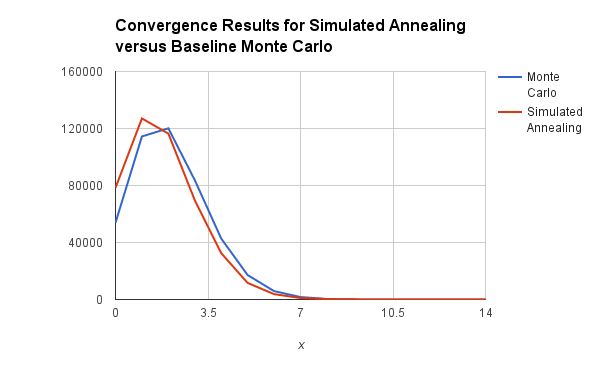
\includegraphics[scale=0.8]{convergence.png}

\section{Results}
%jeremy@mint2 ~/Documents/comp150bg/comp_bio_final_project $ python count_enrichment_dir.py 100_random_enrich/
%0.647129186603 0.0370813397129 28.4736842105, 44
%jeremy@mint2 ~/Documents/comp150bg/comp_bio_final_project $ python count_enrichment_dir.py 100_enrich/
%0.597336658156 0.0313344465786 27.0727272727, 45.6
%jeremy@mint2 ~/Documents/comp150bg/comp_bio_final_project $ python count_enrichments.py %../genecentric/results/yeast_filtered.gobpm 
%(0.9393939393939394, 0.4090909090909091, 62.0, 66)

\par It is not entirely clear how to compare genecentric to simulated annealing. This is because genecentric, which allows for genes to be in mulitple modules, obviously results in more, higher quality modules than simulated annealing. Ultimately, we decided to lean on the percentage of BPMs enriched and percent of BPMs enriched for same function to standardize these measurements. 

\par This line of thought led us to the conclusion that we would need a random group, where BPMs were randomly generated, to compare our results to. Each random group contained about 22 BPMs where each module contained 15 random genes. The average enrichment over many random trials would form a baseline. In the end, we took the average over 59 trials.

\par Additionally, to account for the apparent lack of convergence in the simulated annealing method, we took the average results over 55 trials.

\par In order to compare these different methods, we examined several different benchmarks. Modules found is the number of modules found between size 3 and 25. Modules enriched is the number of modules enriched for at least one GO term at  $p \leq 0.05 $. BPMs Enriched for Same Function is the number of BPMs where both modules had at least one shared GO term.




\begin{table}
    \begin{center}
       \begin{tabular}{ |c | c |c| c | } 
 \hline
 Method & Modules Found & Modules Enriched & BPMs Enriched for Same Function \\
	\hline
 Genecentric              & 66 & 62 (94\%) & 27 (41\%)\\ 
	\hline 
 Simulated Anneal Average & 45.6 & 27.1 (59.7\%) & 1.4 (0.031\%)\\ 
 \hline
 Random Partition Average & 44.0 & 28.44 (64.7\%) & 1.77 (0.040\%)\\ 
 \hline
\end{tabular}
        \caption{Results}\label{tab:results}
    \end{center}
\end{table}
\par This data is particuarly telling. As anticipated, genecentric performed very well. Consequently, our method clearly did not, performing at the same level as completely random selection. This will be explored further in the discussion section.



\section{Discussion}
\par Table \ref{tab:results} cleary shows that our method, simulated annealing, does not produce significant results. We have identified two explanations for this.

\par First, we suspect that we did not run simulated annealing long enough for it to converge. Our data was generated with 50,000 iterations per run. We chose this number because it allowed reasonable fast results and iteration on our internal method. The sample space of this problem is massive. Moreover, individual moves do not result in large changes in the sample space. It thus seems reasonable that we did not come close to fully exploring the sample space.

\par Second, it is pretty clear that the objective function we chose was flawed. Early iterations of the objective function led to either very large or very small modules. Many of these modules were pruned because we opted to not accept groups less than size 3 or greater than size 25. Pruning these modules is not good because we did not allow for repetition of genes between BPM. Thus, by pruning a BPM all genes contained in that BPM are discarded. 

\par In order to fix this, we decided to multiple by a scaling factor to weight against small and large groups. While this scaling factor was effective at limiting large/small groups, it does seem inherently dubious. By scaling around size 30, we mask BPMs that are much smaller or large than that. It seems that this scaling factor would encourage either trimming large BPMs or bloating smaller BPMs. 

\par In theory, an ideal objective function would be able to identify BPMs or many different sizes. However, this objective function is also constrained by runtime. A good objective function will not work in simulated annealing if it takes a long time to run, because it must be run for every iteration. We clearly never found this objective function.

\section{Lessons Learned}
\par Throughout the course of this project, we identified several issues with our approach. The problems prevented us from recognizing the lack of promise in simulated annealing until very late. Each of these problems taught us a lesson about data science in general. 

\par First, starting a data science project, the first priority is figuring out what you are testing against and what you need to do to find significanct results. During this project, one of the last things that we did was run Monte Carlo simulations to get an understanding of what the baseline of success is. It was at this point that we realized that our model was doing about as well as a completely random model. If we knew what this baseline looked like to begin with, then we would have had a better shot at actually beating it.

\par Second, when iterating or tuning a model, you should based on significant parameters. While designing our objective function, we judged the performance of the objective function by visual inspect of the outputed BPMs. A good objective function produced BPMs that contained modules of size between 3 and 25. While these are certainly characteristics of a good BPM, they are more secondary characteristics. We should have appealed directly to enrichment data to see how well an objective function performed. 
		
\par Third, when building a model, it is worth the effort to build infrastructure to store the results of your model in a files. This lets you easily run analytics against results without having to rerun the entire model. While we eventually wrote code for this, we did so very late in the game. In retrospect, the first thing that we should have done is figured out what our data actually looks like throughout our pipeline and written code to move each of those data formats to and from files.

		
	
  


\section{References}
Collins S. Miller K. Maas N., et al. Functional dissection of protein complexes involved in yeast chromosome biology using a genetic interaction map. Nature. 2007;446:806–810.\\

M. Leiserson, D. Tatar, L. Cowen and B. Hescott, "Inferring Mechanisms of Compensation from E-MAP and SGA Data Using Local Search Algorithms for Max Cut," Recomb 2011, pp. 154-167.\\

Gallant, Leiserson, Kackalov, Cowen and Hescott, "Genecentric: A package to uncover graph-theoretic structure in high-throughput epistasis data." BMC Bioinformatics in press, 2013.\\

Berriz G. King O. Bryant B., et al. Characterizing gene sets with funcassociate. Bioinformatics. 2003;19:2502–2504.\\

Simanneal package: https://github.com/perrygeo/simanneal\\

\end{document}
% End of v2-acmlarge-sample.tex (March 2012) - Gerry Murray, ACM
